\section{Silicon in oxide}

\begin{frame}
\tableofcontents[currentsection]
\end{frame}

\begin{frame}
\frametitle{Formulazione problema}

\begin{columns}
\begin{column}{0.5\textwidth}
\begin{equation*}
\begin{cases}
\nabla \cdot ( -\epsilon_0 \epsilon_r \nabla \varphi) = q(p-n+D) & \text{in $\Omega_{Si}$}\\
\nabla \cdot ( -\epsilon_0 \epsilon_r \nabla \varphi) = 0 & \text{in $\Omega_{Ox}$}\\
\nabla \varphi \cdot \vect{n} =0 & \text{su $\Gamma_{Ox}$ }\\
\varphi = \varphi_K & \text{su $\Gamma_{K}$}\\
\varphi = \varphi_A & \text{su $\Gamma_{A}$}\\
\end{cases}
\end{equation*}
\end{column}
\end{columns}

\begin{center}
\begin{tikzpicture}
[scale=1.5]

\draw [thick] (2,0) rectangle (3,1);
\node at (-0.25,1.25) {$\Gamma_{A}$};
\node at (3.3,0.5) {$\Gamma_{K}$};
\node at (2,1.75) {$\Gamma_{Ox}$};
\node at (1,1) {$\Omega_{Si}$};
\node at (0.4,0.4) {$\Omega_{Ox}$};


\draw [thick] (2,1)--(0,2)--(1,2)--(3,1);
\draw [thick] (2,0)--(0,1)--(0,2);

%\draw [dashed,thick] (0,1)--(1,1)--(1,2);
%\draw [dashed,thick] (1,1)--(3,0);

\draw [pattern=north west lines, pattern color=gray, thick] (2.1,0.1) rectangle (2.9,0.9);


\draw [dashed] (0.1,1.1) rectangle (0.9,1.9);
\draw [dashed] (2.9,0.1)--(0.9,1.1);
\draw [dashed] (2.9,0.9)--(0.9,1.9);
\draw [dashed] (2.1,0.1)--(0.1,1.1);
\draw [dashed] (2.1,0.9)--(0.1,1.9);
%\draw [thick,dashed] (2.9,0.1)--(0.9,1.1);

\end{tikzpicture}

\end{center}
\end{frame}

\begin{frame}
\frametitle{Newton}

\begin{equation*}
\begin{cases}
-\nabla \cdot ( \epsilon_{Si} \nabla \delta\varphi) + \sigma\delta\varphi = \nabla \cdot ( \epsilon_{Si} \nabla \varphi) + q(p-n+D) & \text{in $\Omega_{Si}$}\\
-\nabla \cdot ( \epsilon_{Ox} \nabla \delta\varphi) = \nabla \cdot ( \epsilon_{Ox} \nabla \varphi) & \text{in $\Omega_{Ox}$}\\
\nabla \delta\varphi \cdot \vect{n} =0 & \text{su $\Gamma_{Ox}$ }\\
\delta\varphi = 0 & \text{su $\Gamma_{K}$}\\
\delta\varphi = 0 & \text{su $\Gamma_{A}$}\\
\end{cases}
\end{equation*}

\begin{alertblock}{Domanda:}
Cosa bisogna imporre, come valore di forzante e coefficiente di reazione, sui nodi di frontiera fra il bulk di silicio e l'ossido?
\end{alertblock}

\end{frame}


\begin{frame}
\frametitle{Sezioni fissate le coordinate X e Z}
\begin{columns}
\begin{column}{0.5 \textwidth}
\begin{center}
Valori al bordo pari al silicio
\begin{figure}[!h]
         \subfigure[Potenziale]
          {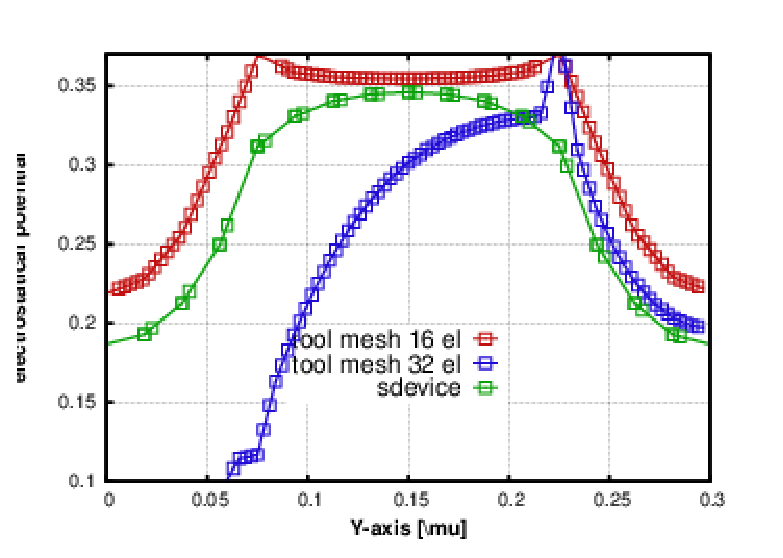
\includegraphics[scale=0.3]{N1e17_P1e17_OX_electro_lineZ002_withsigma}}
	\subfigure[Carica]
	  {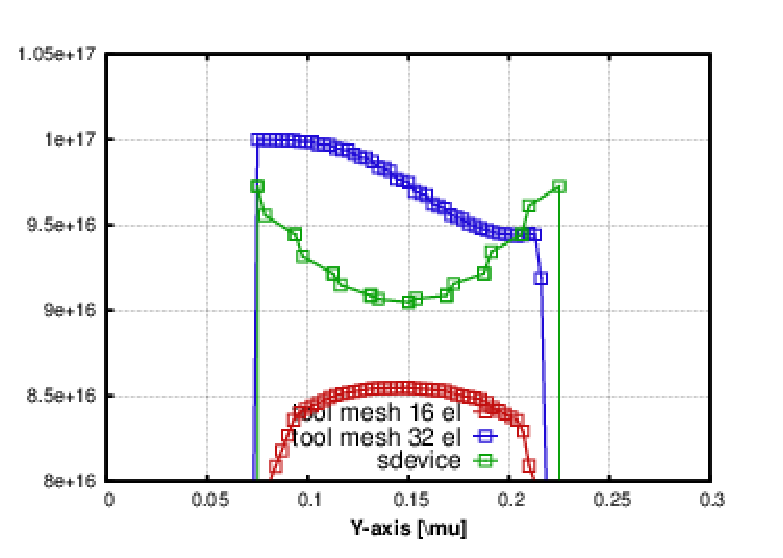
\includegraphics[scale=0.3]{N1e17_P1e17_OX_spacecharge_lineZ002_withsigma}}
\end{figure}
\end{center}
\end{column}
\begin{column}{0.5 \textwidth}
\begin{center}
Valori al bordo pari all'ossido
\begin{figure}[!h]
         \subfigure[Potenziale]
          {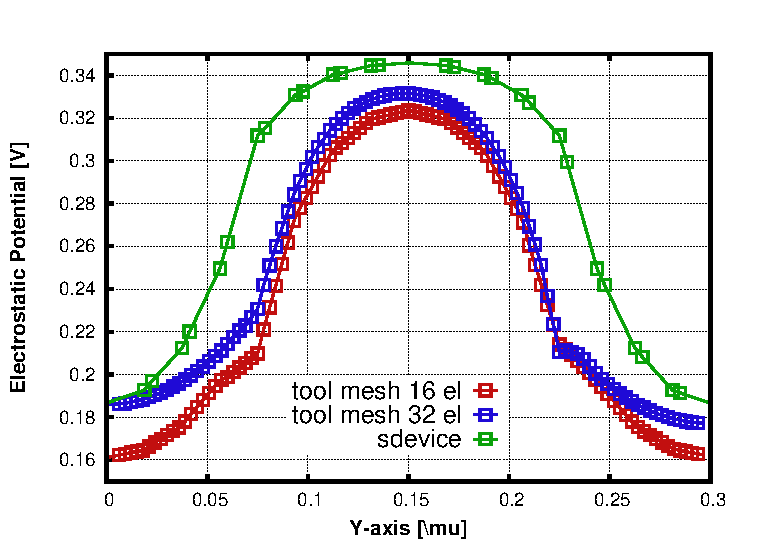
\includegraphics[scale=0.3]{N1e17_P1e17_OX_lineZ002}}
	\subfigure[Carica]
	  {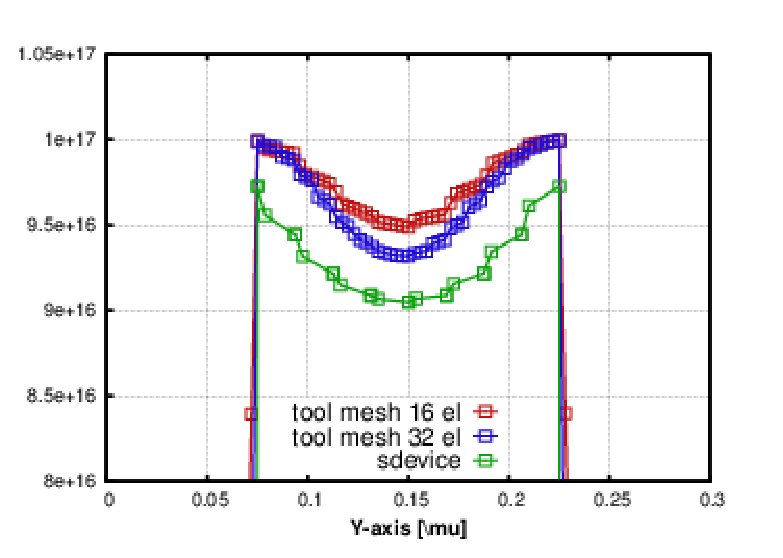
\includegraphics[scale=0.3]{N1e17_P1e17_OX_spacecharge_lineZ002}}
\end{figure}
\end{center}
\end{column}
\end{columns}

\end{frame}


\begin{frame}
\frametitle{Decisione empirica}
\begin{itemize}
\item[1.] Le soluzioni non coincidono pi\`u con sdevice
\item[2.] La scelta di imporre i valori relativi all'ossido sembra portare la soluzione pi\`u vicina ad sdevice 
\end{itemize}
Nei test successivi adottiamo la scelta di valori pari all'ossido sull'interfaccia.
\end{frame}

\subsection{N16P16}
\begin{frame}
\tableofcontents[currentsection]
\end{frame}

\begin{frame}
\frametitle{Asimmetria-Potenziale N16P16}
Evidente asimmetria fra le differenti sezioni e problema allineamento valore di interfaccia sulla frontiera ossido silicio.
\begin{columns}

\begin{column}{0.3 \textwidth}
\begin{center}
\begin{figure}[!h]
         \subfigure[Sezione XZ]
          {\includegraphics[scale=0.18]{N16P16OX_POT_tool_XZ}}
          \end{figure}
\end{center}
\end{column}

\begin{column}{0.3 \textwidth}
\begin{center}
\begin{figure}[!h]
         \subfigure[Sezione YZ]
          {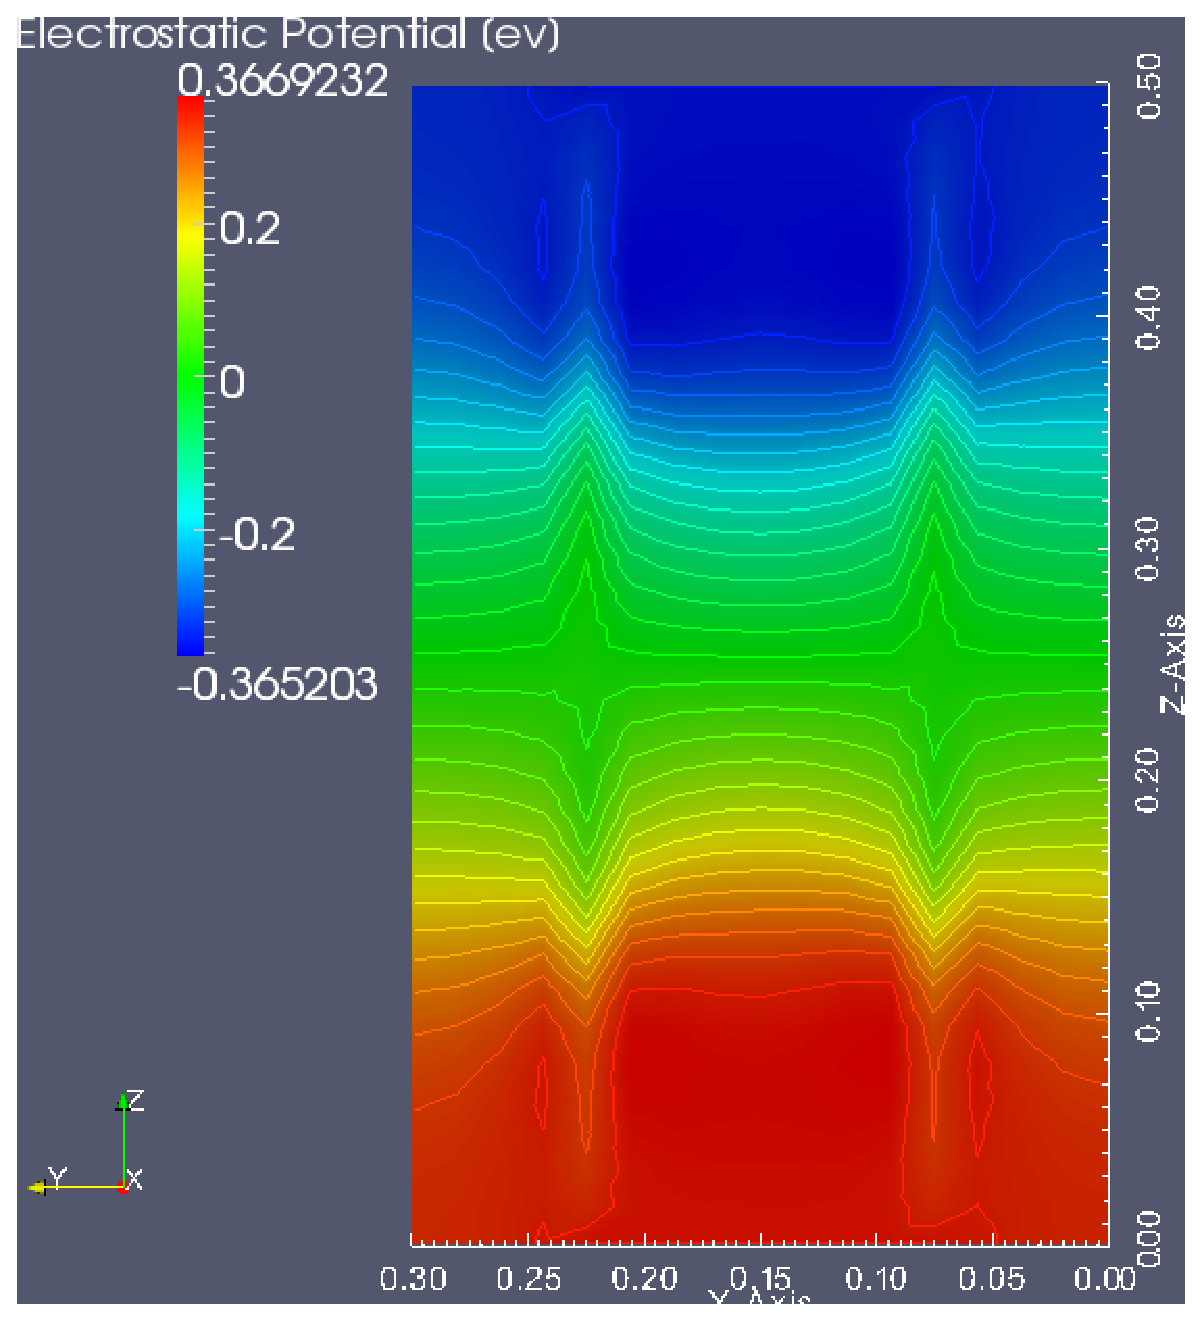
\includegraphics[scale=0.18]{N16P16OX_POT_tool_YZ}}
\end{figure}
\end{center}
\end{column}

\begin{column}{0.3 \textwidth}
\begin{center}
\begin{figure}[!h]
         \subfigure[Sdevice]
          {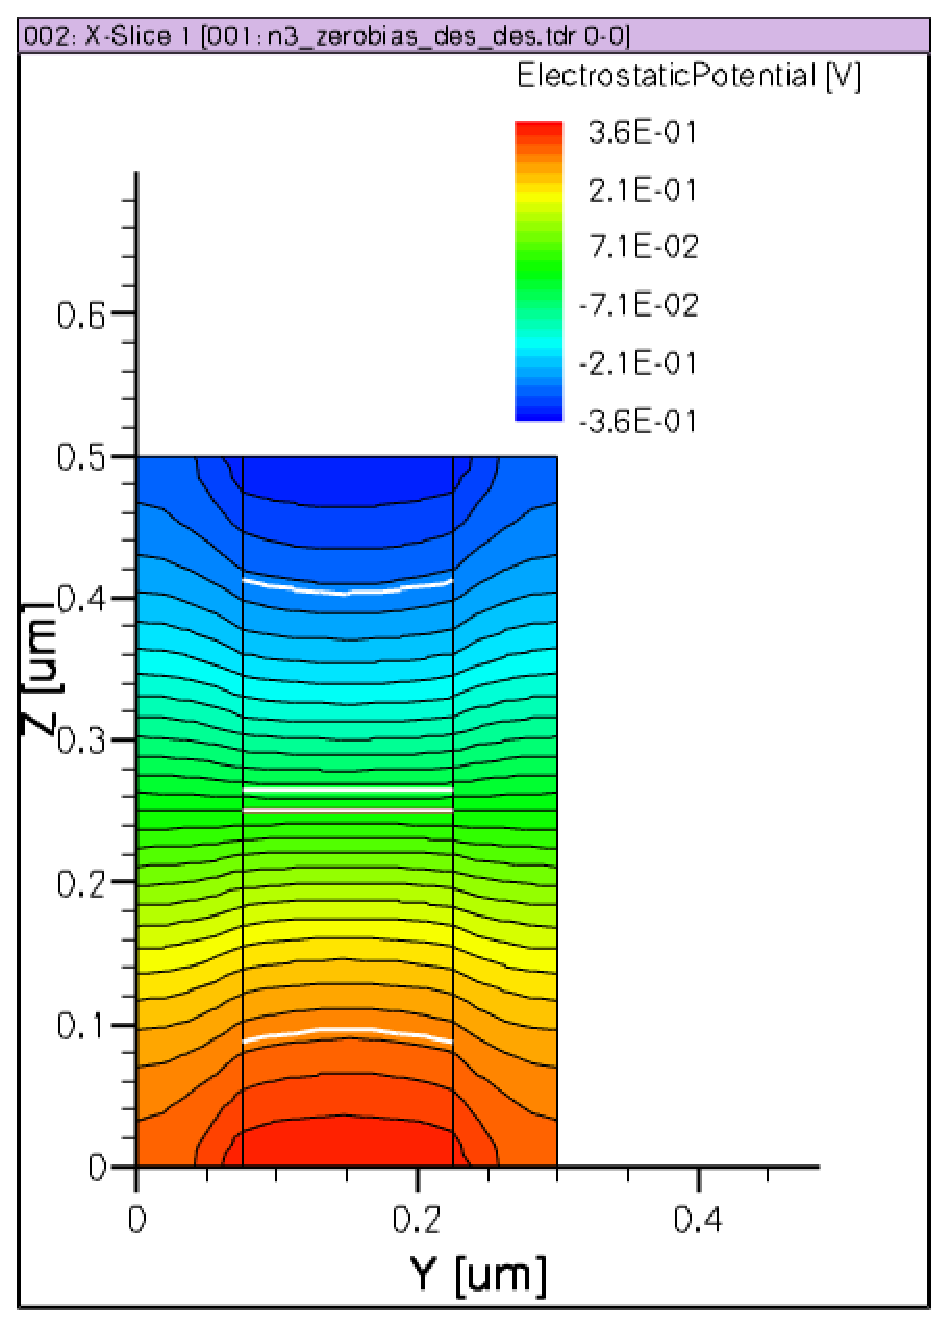
\includegraphics[scale=0.18]{N16P16OX_POT_sdevice_YZ}}
\end{figure}
\end{center}
\end{column}

\end{columns}

\end{frame}



\begin{frame}
\frametitle{Picchi inaspettati - Free Charge N16P16}
Valori numerici nella prima parte di zona svuotata soddisfacienti. Cambiamento di tendenza avvicinandosi ai contatti. Instabilit\`a?Condizioni di bordo applicate male?
\begin{columns}

\begin{column}{0.5 \textwidth}
\begin{center}
\begin{figure}[!h]
          {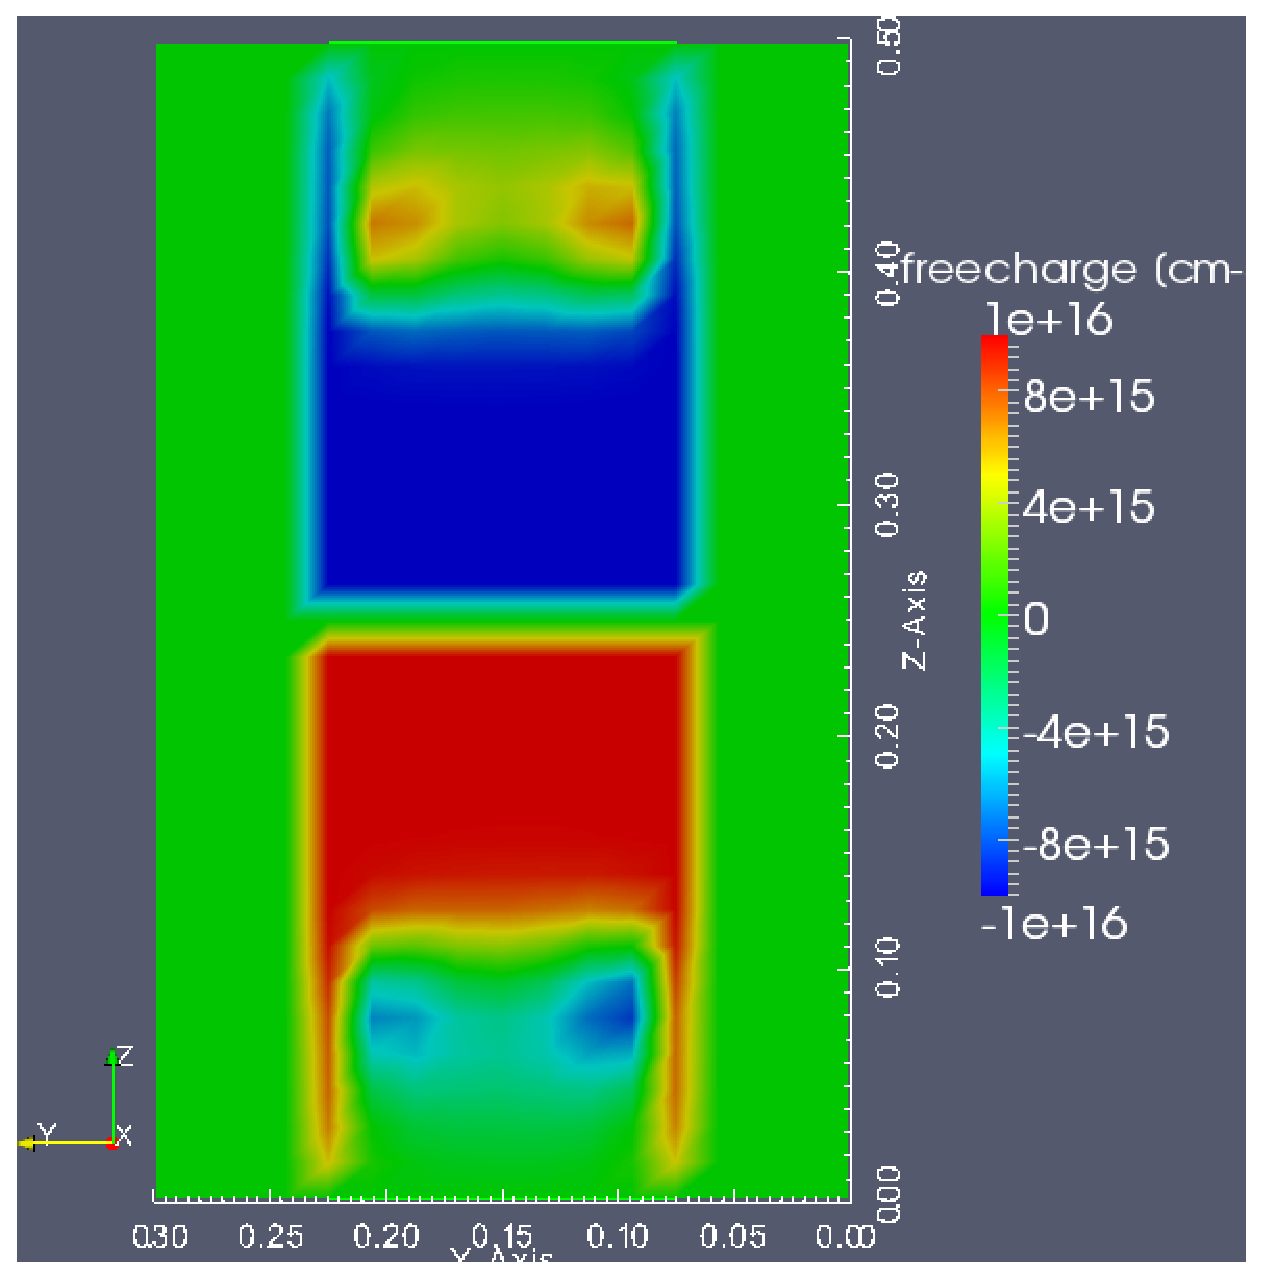
\includegraphics[scale=0.25]{N16P16OX_Q_tool_YZ}}
          \end{figure}
\end{center}
\end{column}

\begin{column}{0.5 \textwidth}
\begin{center}
\begin{figure}[!h]
          {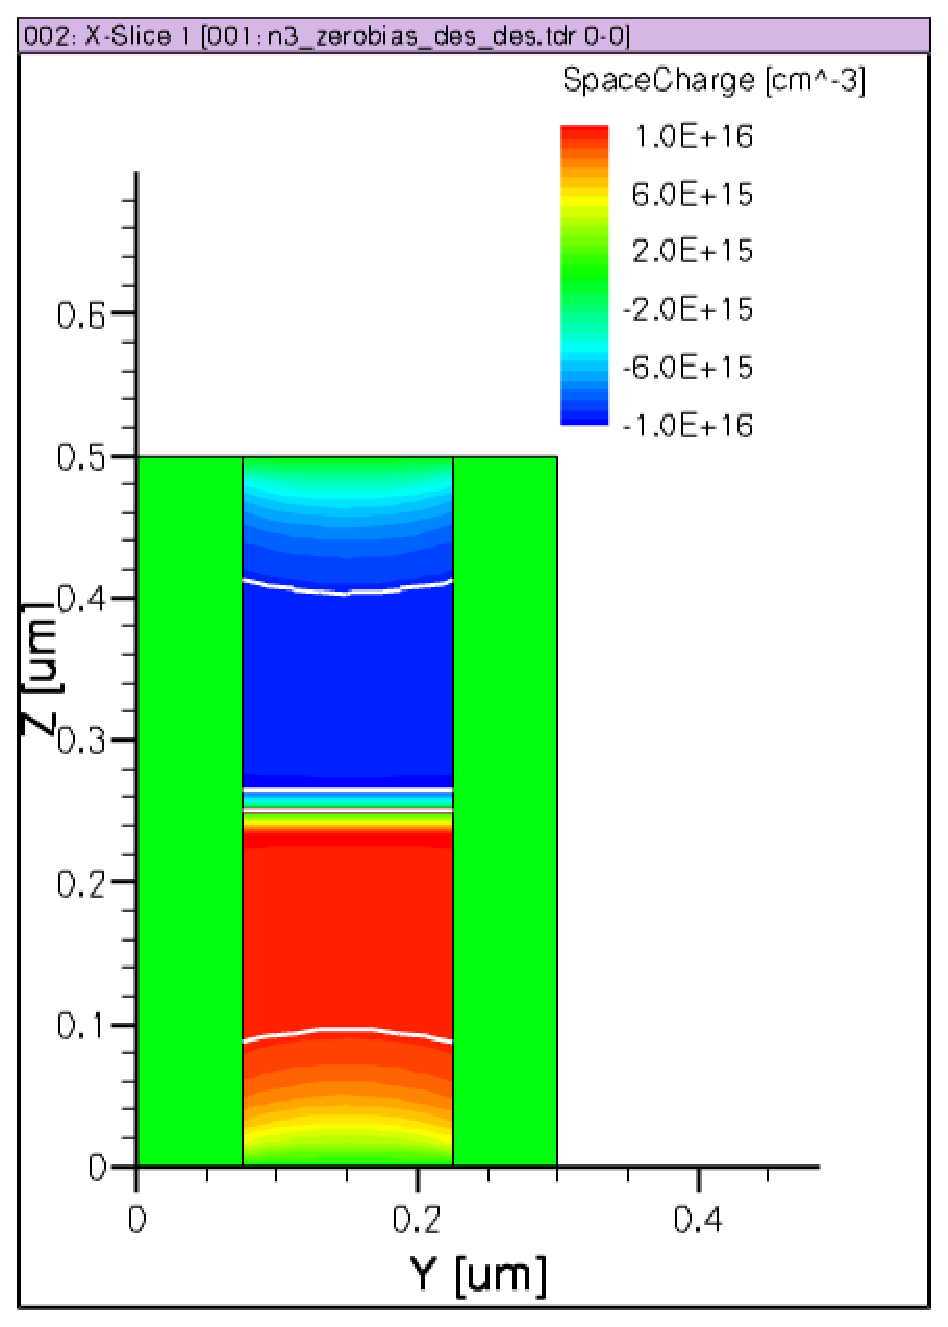
\includegraphics[scale=0.25]{N16P16OX_Q_sdevice_YZ}}
\end{figure}
\end{center}
\end{column}

\end{columns}

\end{frame}

\subsection{N17P17}
\begin{frame}
\tableofcontents[currentsection]
\end{frame}

\begin{frame}
\frametitle{Asimmetria - Potenziale N17P17}
Asimmetria accentuata (o forse prima era mascherata dai problemi di interfaccia?). Sovraddiffusione del potenziale all'interno dell'ossido.
\begin{columns}

\begin{column}{0.3 \textwidth}
\begin{center}
\begin{figure}[!h]
\subfigure[Sezione XZ]
          {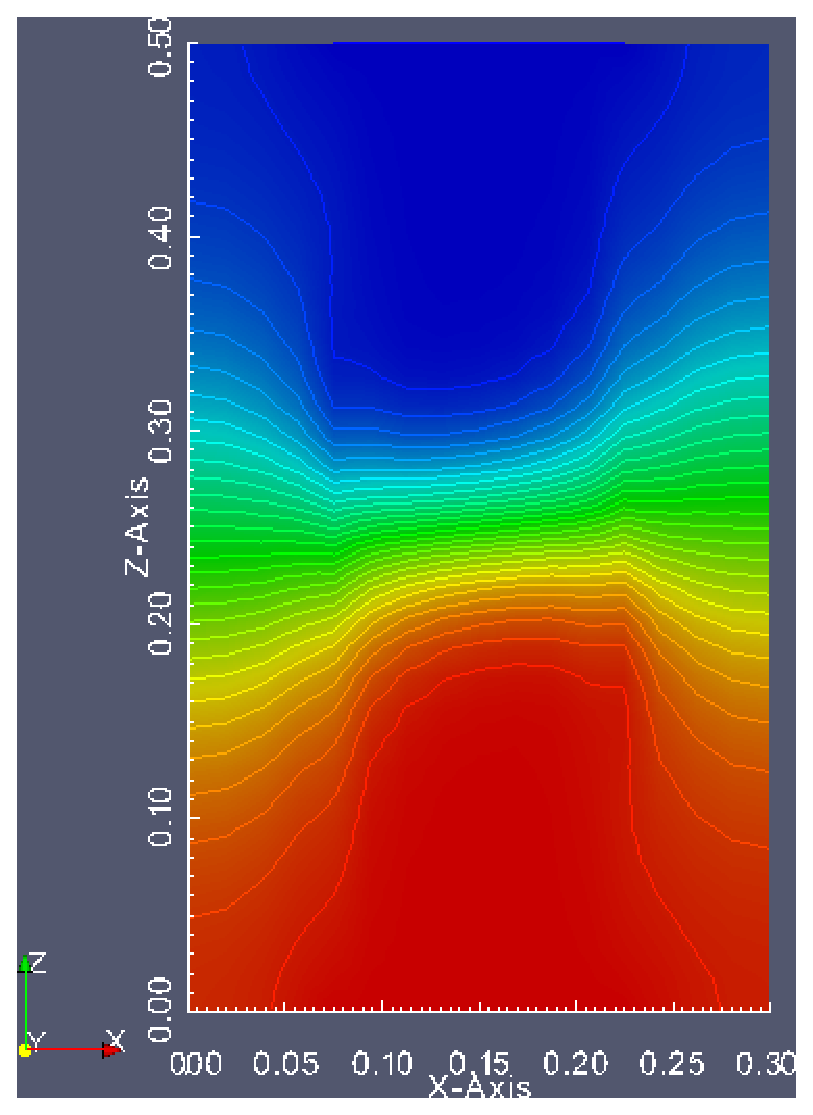
\includegraphics[scale=0.2]{N17P17OX_POT_tool_XZ}}
          \end{figure}
\end{center}
\end{column}

\begin{column}{0.3 \textwidth}
\begin{center}
\begin{figure}[!h]
\subfigure[Sezione YZ]
          {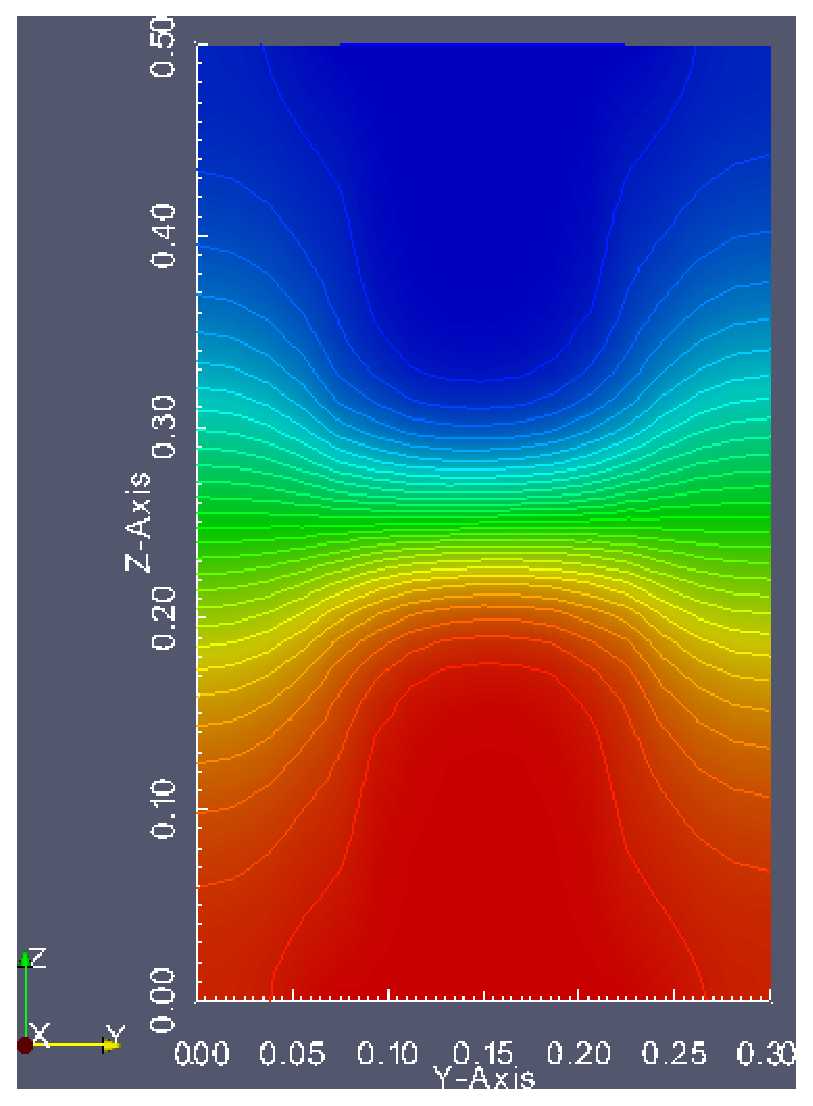
\includegraphics[scale=0.2]{N17P17OX_POT_tool_YZ}}
\end{figure}
\end{center}
\end{column}

\begin{column}{0.3 \textwidth}
\begin{center}
\begin{figure}[!h]
\subfigure[Sdevice]
          {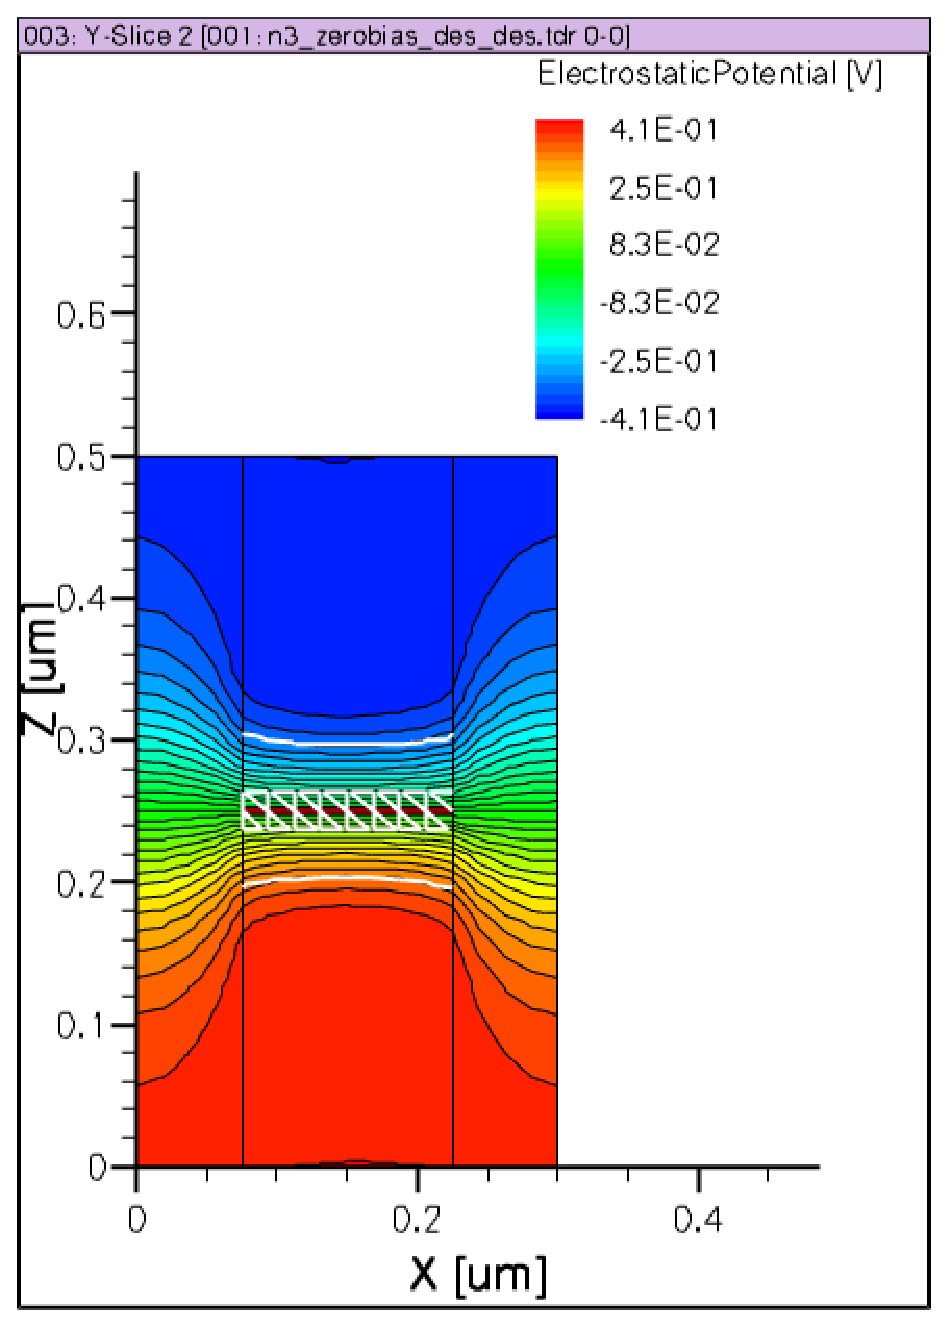
\includegraphics[scale=0.2]{N17P17OX_sdevice_XZ}}
\end{figure}
\end{center}
\end{column}

\end{columns}

\end{frame}




\begin{frame}
\frametitle{Asimmetria - Free Charge N17P17}
Ripercussioni della asimmetria evidenti sulla carica. Migliore grafico ottenuto per valori e distribuzione (l'apporto sovradiffusivo si fa notare allungando maggiormente le code di zona svuotata)
\begin{columns}

\begin{column}{0.3 \textwidth}
\begin{center}
\begin{figure}[!h]
\subfigure[Sezione XZ]
          {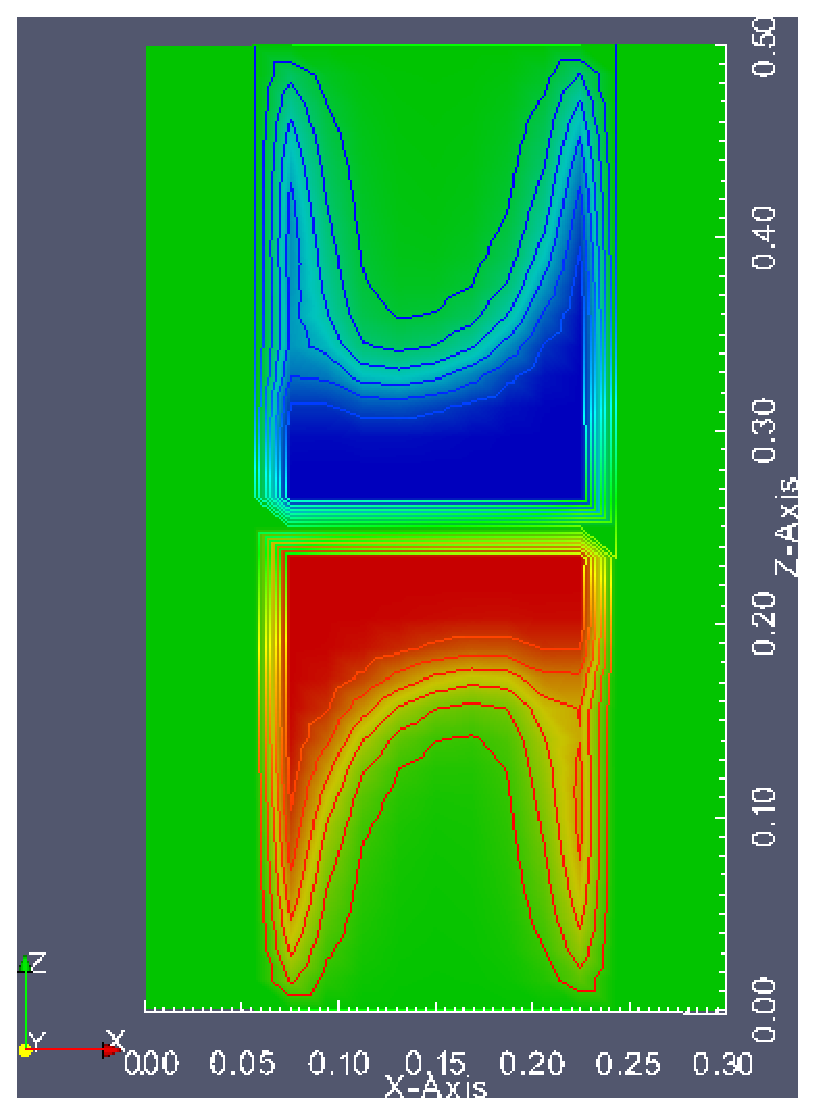
\includegraphics[scale=0.2]{N17P17OX_Q_tool_XZ}}
          \end{figure}
\end{center}
\end{column}

\begin{column}{0.3 \textwidth}
\begin{center}
\begin{figure}[!h]
\subfigure[Sezione YZ]
          {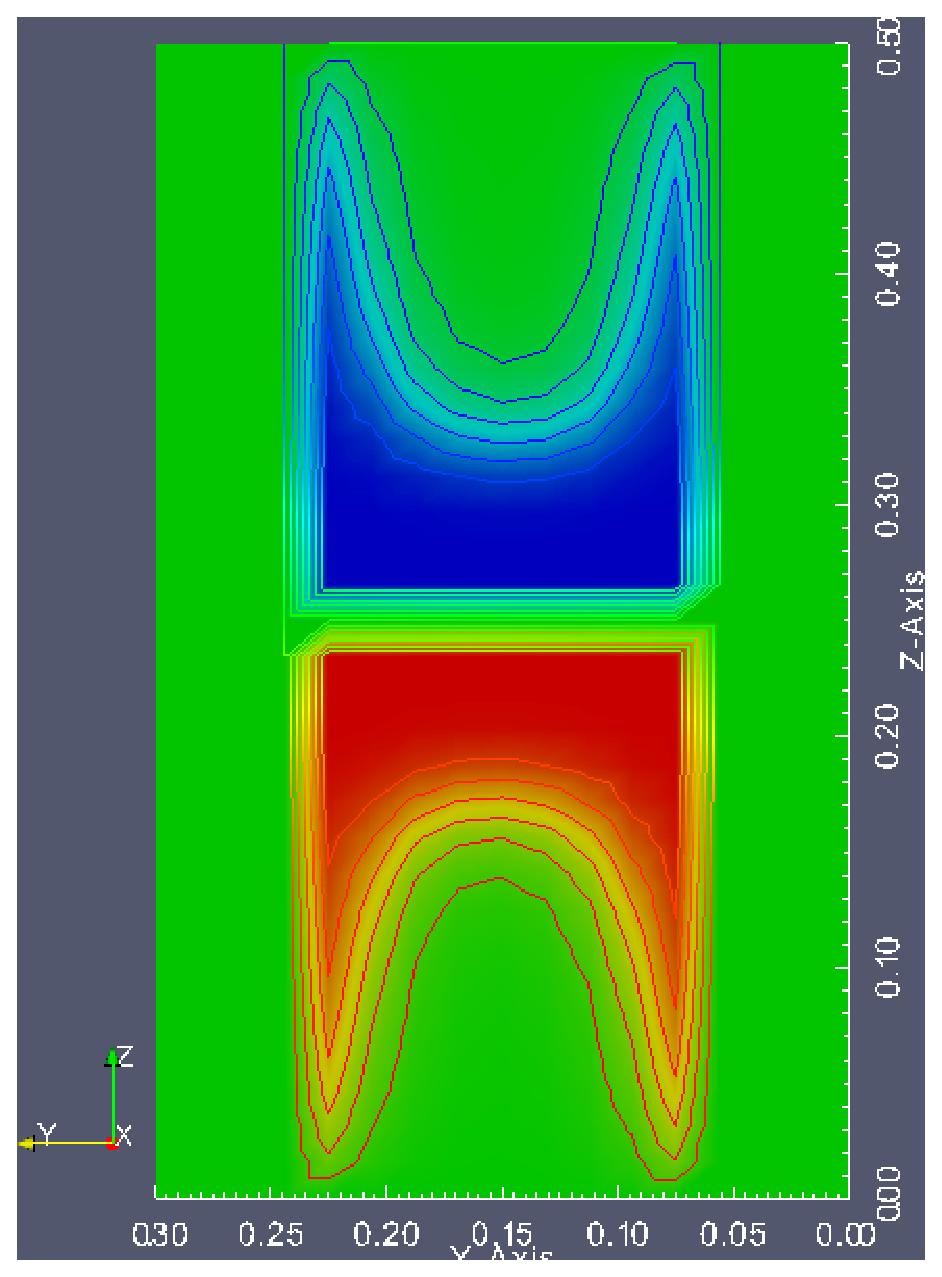
\includegraphics[scale=0.2]{N17P17OX_Q_tool_YZ}}
\end{figure}
\end{center}
\end{column}

\begin{column}{0.3 \textwidth}
\begin{center}
\begin{figure}[!h]
\subfigure[Sdevice]
          {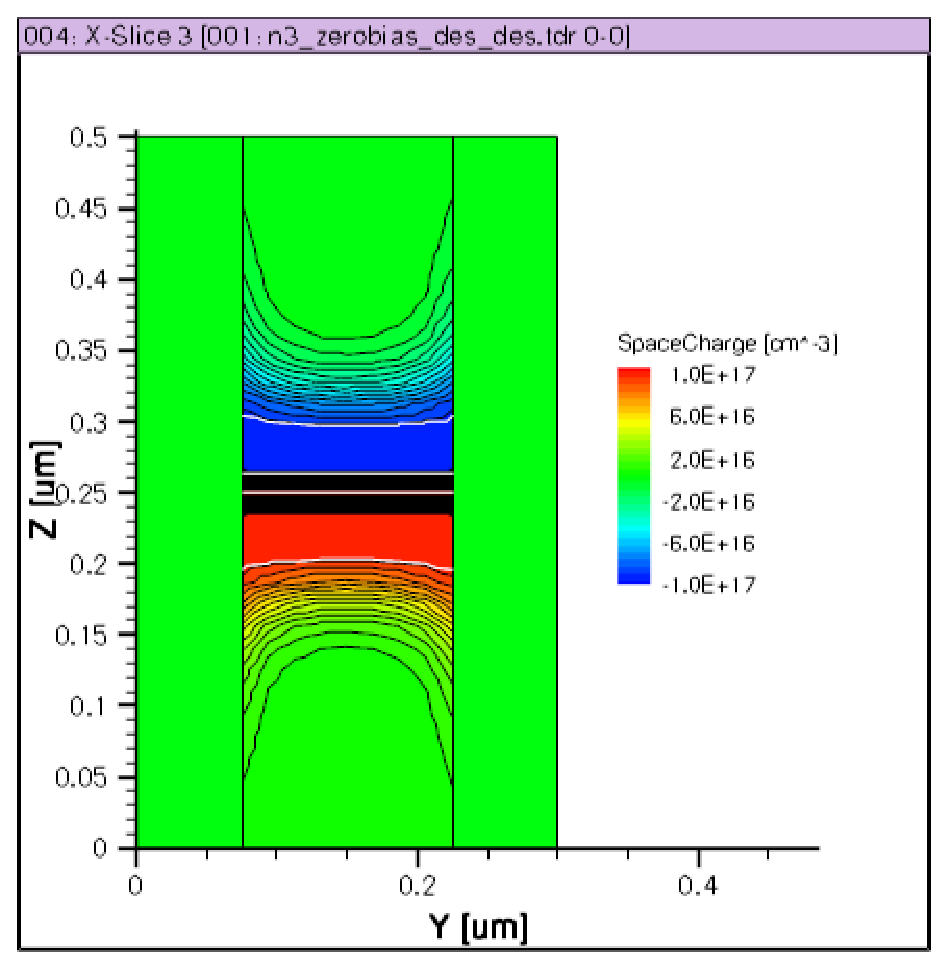
\includegraphics[scale=0.2]{N17P17OX_Q_sdevice_YZ}}
\end{figure}
\end{center}
\end{column}

\end{columns}

\end{frame}

\subsection{N19P19}
\begin{frame}
\tableofcontents[currentsection]
\end{frame}

\begin{frame}
\frametitle{Asimmetria scomparsa - Potenziale  N19P19}
Smorzamento dell'asimmetria dei risulatati, probabilmente dovuto al drogaggio alto (che rendendo pi\`u fine la zona svuotata non permette di valutare un'eventuale asimmetria). Fenomeno di sovraddiffusione contenuto (o assente?) probabilmente per la medesima motivazione.
\begin{columns}

\begin{column}{0.3 \textwidth}
\begin{center}
\begin{figure}[!h]
\subfigure[Sezione XZ]
          {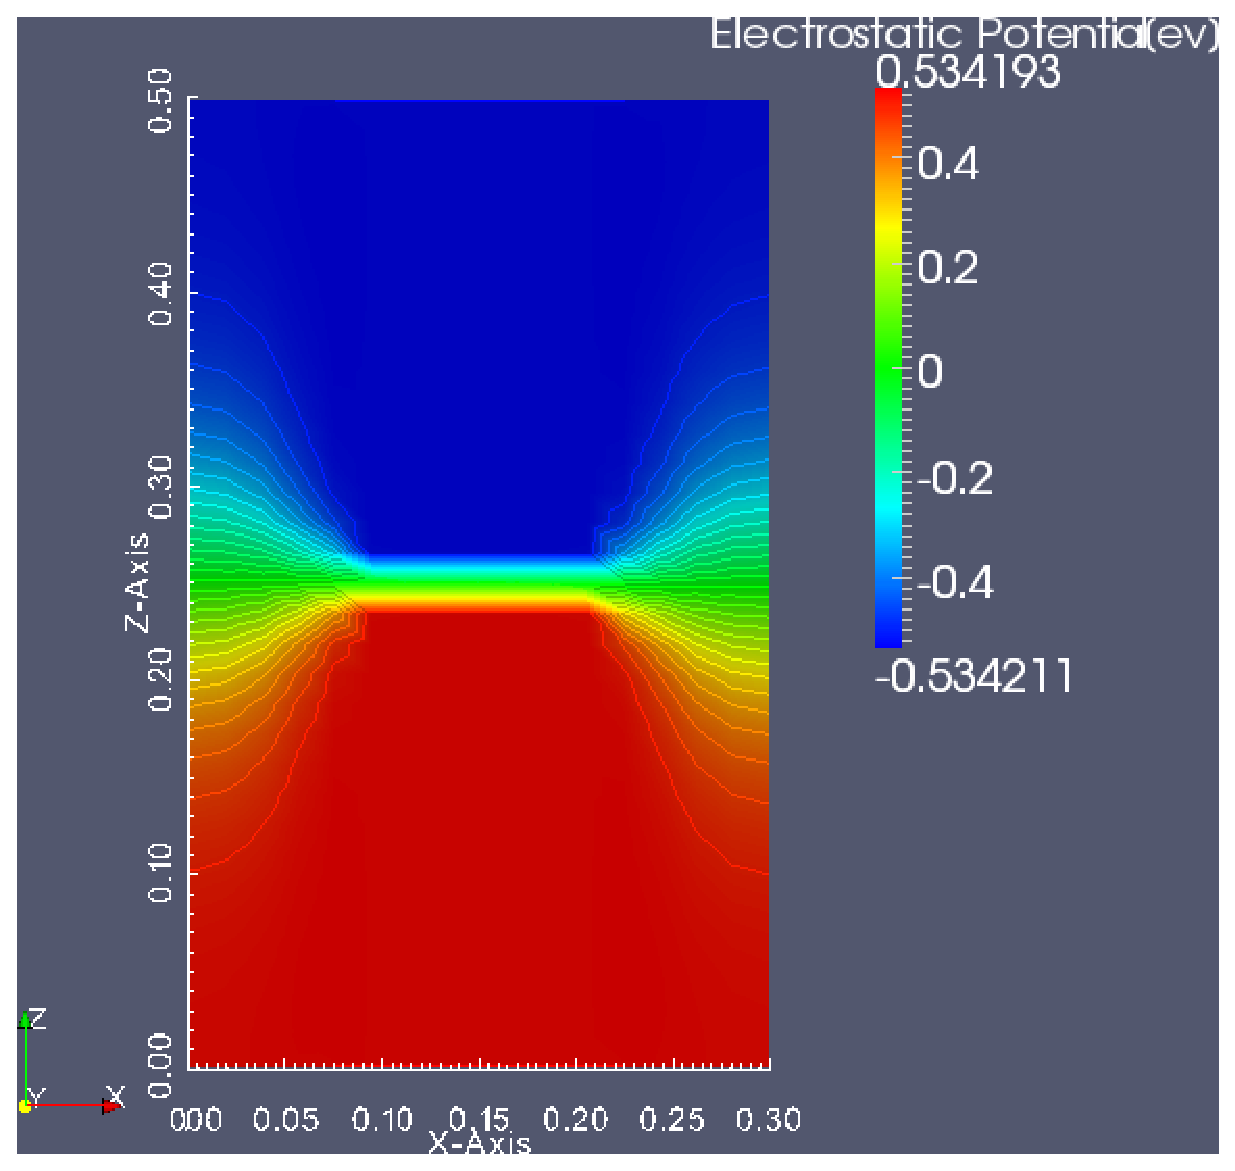
\includegraphics[scale=0.2]{N19P19OX_POT_tool_XZ}}
          \end{figure}
\end{center}
\end{column}

\begin{column}{0.3 \textwidth}
\begin{center}
\begin{figure}[!h]
\subfigure[Sdevice]
          {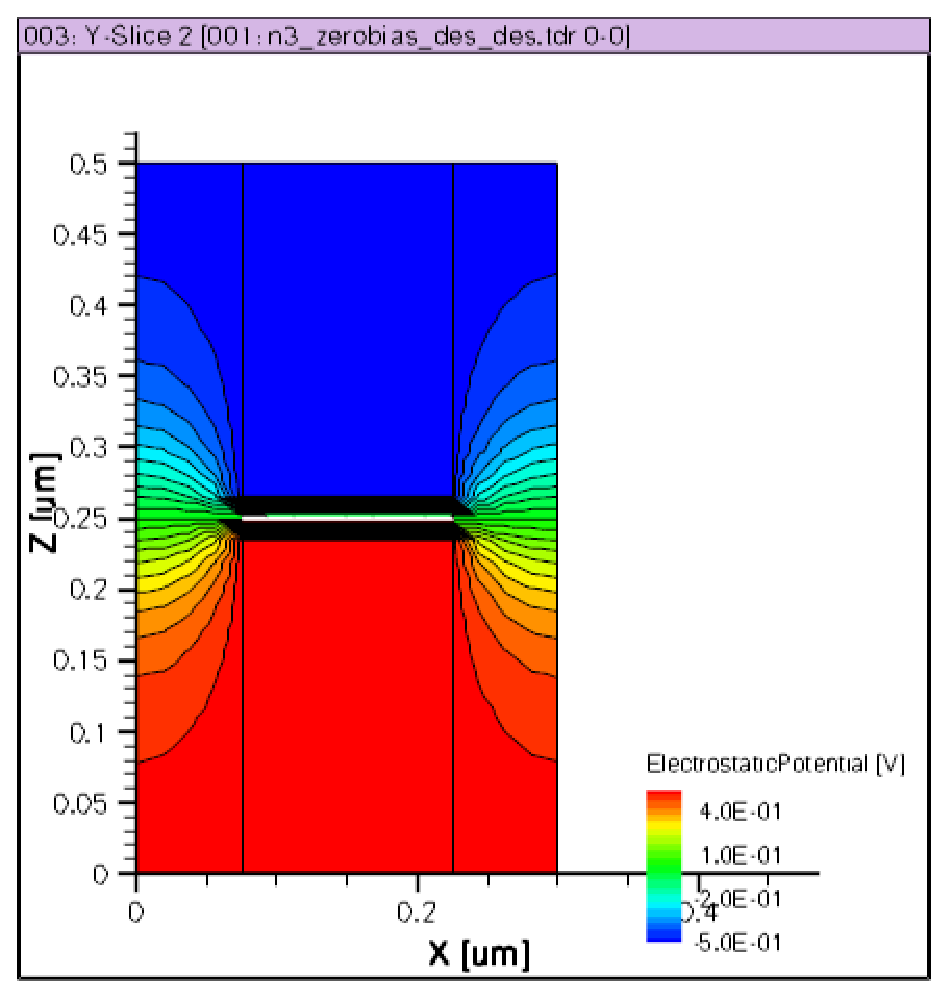
\includegraphics[scale=0.2]{N19P19OX_POT_sdevice_XZ}}
\end{figure}
\end{center}
\end{column}

\end{columns}

\end{frame}

\begin{frame}
\frametitle{Carica interfacciale - Free Charge N19P19}
Problemi evidenti di carica interfacciale nonostante la soluzione del potenziale sembra essere quella che si avvicini di pi\`u alla soluzione sdevice.
\begin{columns}

\begin{column}{0.3 \textwidth}
\begin{center}
\begin{figure}[!h]
\subfigure[Sezione XZ]
          {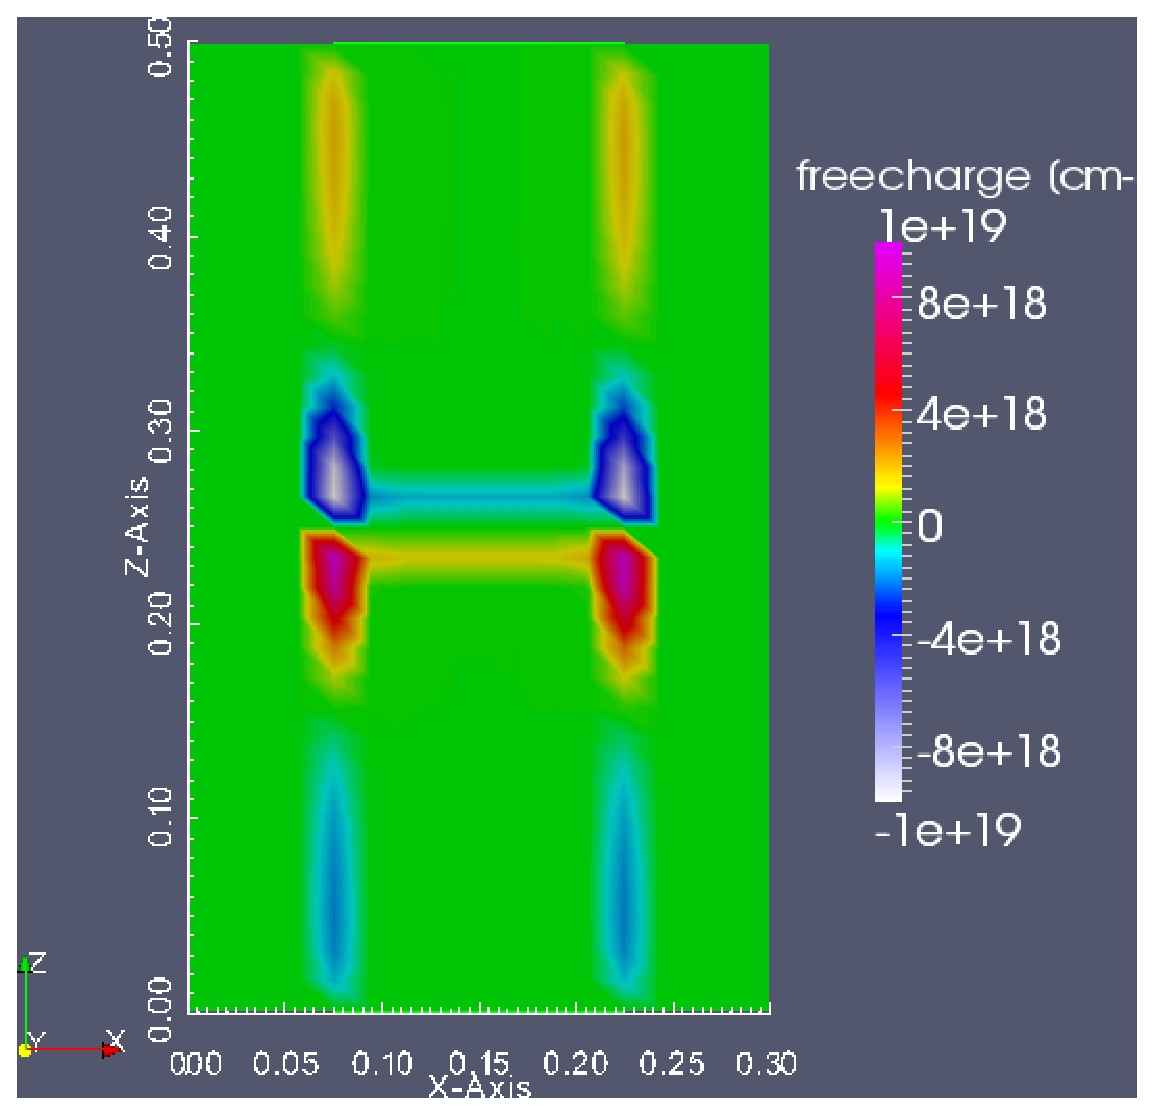
\includegraphics[scale=0.2]{N19P19OX_Q_tool_XZ}}
          \end{figure}
\end{center}
\end{column}

\begin{column}{0.3 \textwidth}
\begin{center}
\begin{figure}[!h]
\subfigure[Sezione YZ]
          {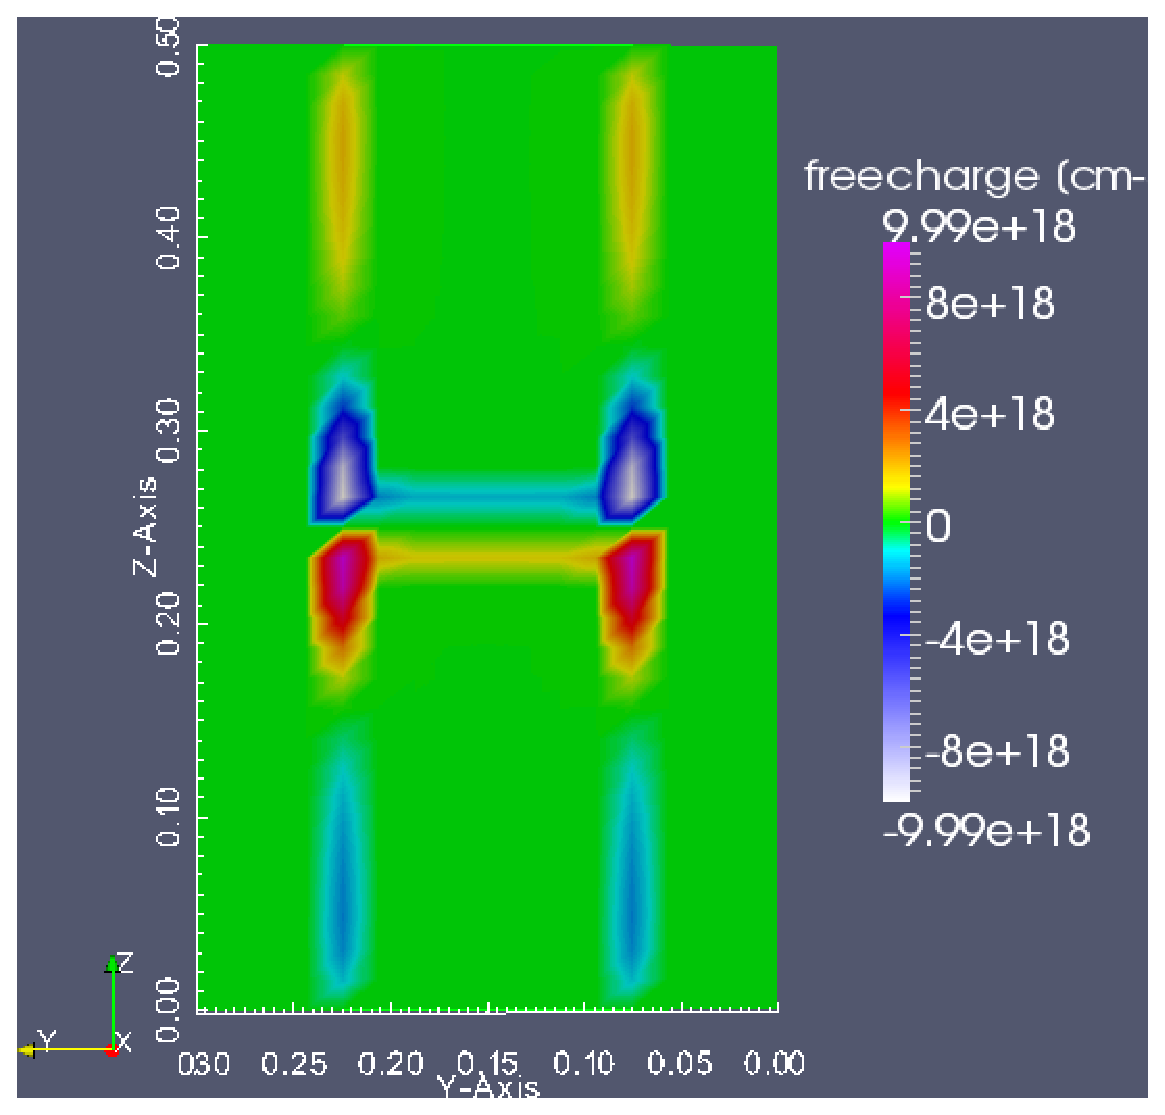
\includegraphics[scale=0.2]{N19P19OX_Q_tool_YZ}}
\end{figure}
\end{center}
\end{column}

\begin{column}{0.3 \textwidth}
\begin{center}
\begin{figure}[!h]
\subfigure[Sdevice]
          {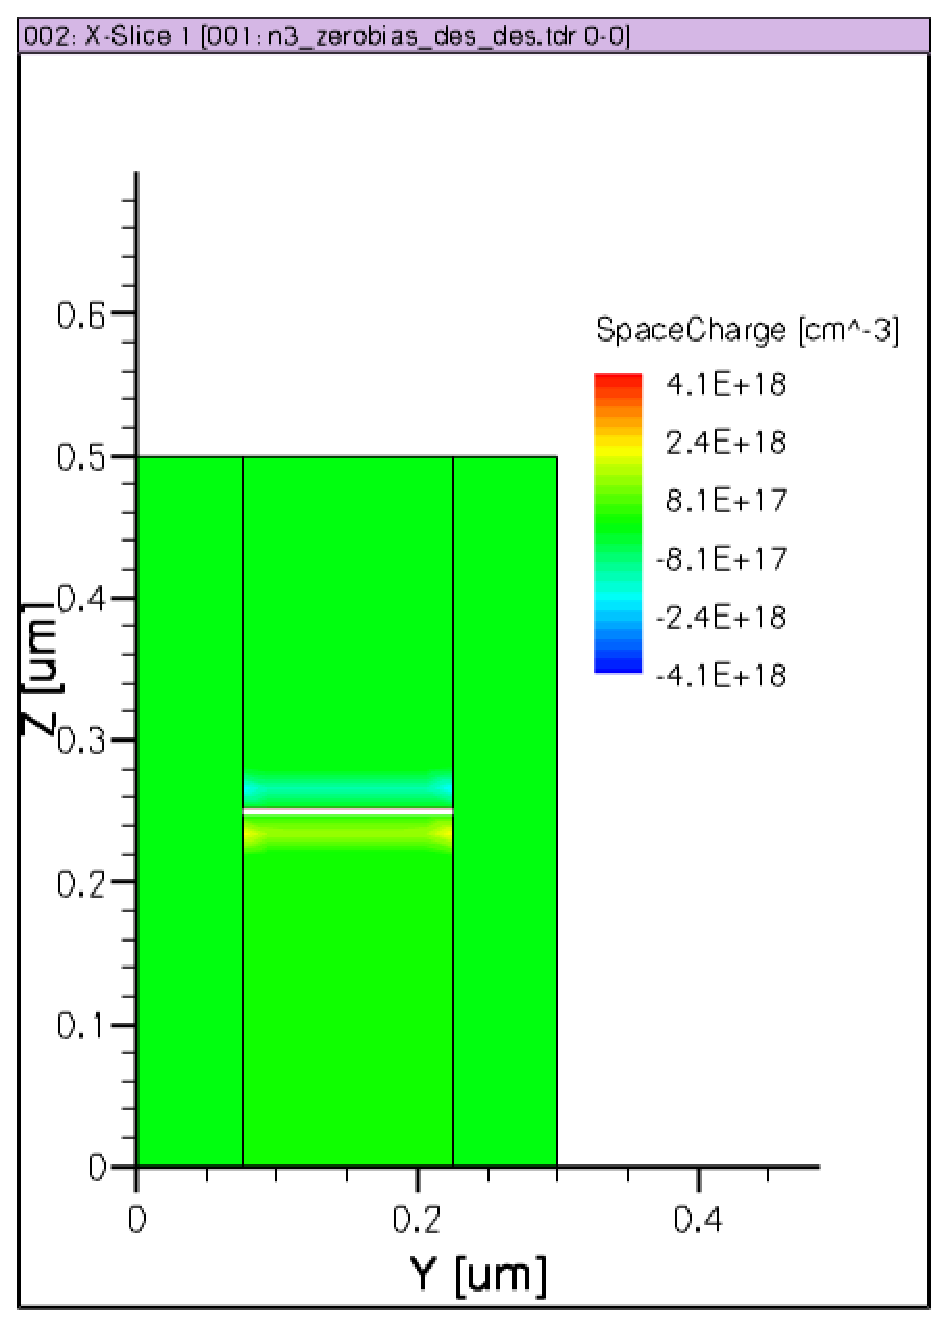
\includegraphics[scale=0.2]{N19P19OX_Q_sdevice_YZ}}
\end{figure}
\end{center}
\end{column}

\end{columns}

\end{frame}


\begin{frame}
\frametitle{Conclusioni}
\begin{itemize}
\item[1.] Il solutore non lineare di Poisson sul silicio \`e allineato con i risultati di sdevice.
\item[2.] Il solutore lineare di Poisson su ossido \`e allineato con i risultati di sdevice
\item[3.] Il solutore non lineare di Poisson applicato alla situazione silicio-ossido non d\`a soluzioni corrette: viste le conclusioni precedenti il problema \`e legato al trattamento dell'interfaccia silicio-ossido. 
\end{itemize}
\end{frame}